\documentclass[12pt, a4paper, notitlepage, onecolumn]{article}

\usepackage[affil-it, blocks]{authblk}
\usepackage[margin=2cm]{geometry}
\usepackage[utf8]{inputenc}
\usepackage[russian]{babel}
\usepackage{setspace}


\usepackage{graphicx}
\usepackage{subcaption}


\onehalfspacing
\renewcommand\Authand{ ~и~}
\renewcommand\Authands{ и }




\begin{document}
\begin{flushright}
УДК {53.082.79}
\end{flushright}
\title{Проектирование детектора протонов и электронов для мониторинга солнечных космических лучей}
\author[1,2,3]{М. Зелёный%
  \thanks{Докладчик: mihail.zelenyy@phystech.edu}}
\author[1,2]{Е. Стадничук}
\author[1,2]{А. Нозик}
\author[3]{И. Зимовец}
\author[1]{А. Кудинов}
\author[1]{И. Резников}
\affil[1]{МФТИ (ГУ), 141701, Московская облаcть,
г. Долгопрудный, Институтский пер., 9.} 
\affil[2]{ИЯИ РАН, 117312, г. Москва, В-312, проспект 60-летия Октября, 7а.}%
\affil[3]{ИКИ РАН, 117997, г. Москва, ул. Профсоюзная 84/32}%

\date{}
{\let\newpage\relax\maketitle}

\begin{abstract}
В докладе представлен проект компактного космического детектора для измерения энергетических спектров протонов (10 -- 100~МэВ) и электронов (до 10~МэВ) в солнечных космических лучах. Детектор может работать в двух режимах: дифференциальном (восстанавливается каждое событие) и интегральном (восстанавливается только энергетический спектр и состав излучения при большой загрузке).
\end{abstract}

{\noindent \bf Ключевые слова:} детектор элементарных частиц, солнечные космические лучи, математическая статистика, анализ данных, компьютерное моделирование. 


\section*{Введение.} 
В результате спорадических явлений солнечной активности, таких как вспышки и корональные выбросов массы, электроны/ионы могут ускоряться до энергий в десятки МэВ/ГэВ соответственно, образуя так называемые  солнечные космические лучи (СКЛ)~\cite{miroshnichenko2015solar}. Несмотря на многолетнее интенсивное исследование СКЛ, остается еще масса неразрешенных вопросов. До сих пор нет окончательного понимания механизмов ускорения частиц, их выхода из солнечной короны и распространения в межпланетной среде ~\cite{miroshnichenko2015solar}. Детальное понимание этих механизмов является фундаментальной задачей, поскольку схожие физические процессы происходят во многих астрофизических объектах. Более того, это требуется для построения надежного количественного прогноза СКЛ в различных точках гелиосферы, поскольку СКЛ могут оказывать серьезное негативное воздействие как на околоземные космические системы и межпланетные станции, так и на биологические объекты на их борту ~\cite{petrukovich2008cosmic}. Развитие космической техники и освоение космического пространства требует прогресса в изучении СКЛ и, в идеале, создание разветвленной сети мониторинговых космических станций. Для этого, в частности, необходимо создание надежных, легких, компактных, потребляющих малую мощность детекторов энергичных частиц, способных одновременно измерять электроны и ионы в диапазонах энергий~1 -- 10~МэВ и~10 -- 100~МэВ соответственно. 

\section*{Описание детектора и методика измерения.}
В работе представлена концепция телескопа на основе сегментированного сцинтилляционного детектора. Методика измерения основана на анализе кривой зависимости ионизационных потерь (см. рис.~\ref{pic-01-a}) от пробега частицы. По этой кривой можно с высокой точностью идентифицировать тип частицы и её кинетическую энергию, в том числе благодаря наличию у протонов характерной особенности --- пика Брэгга в конце кривой ~\cite{Gruppen}.
\begin{figure}[ht!]
	\begin{subfigure}[b]{0.5\textwidth}
    	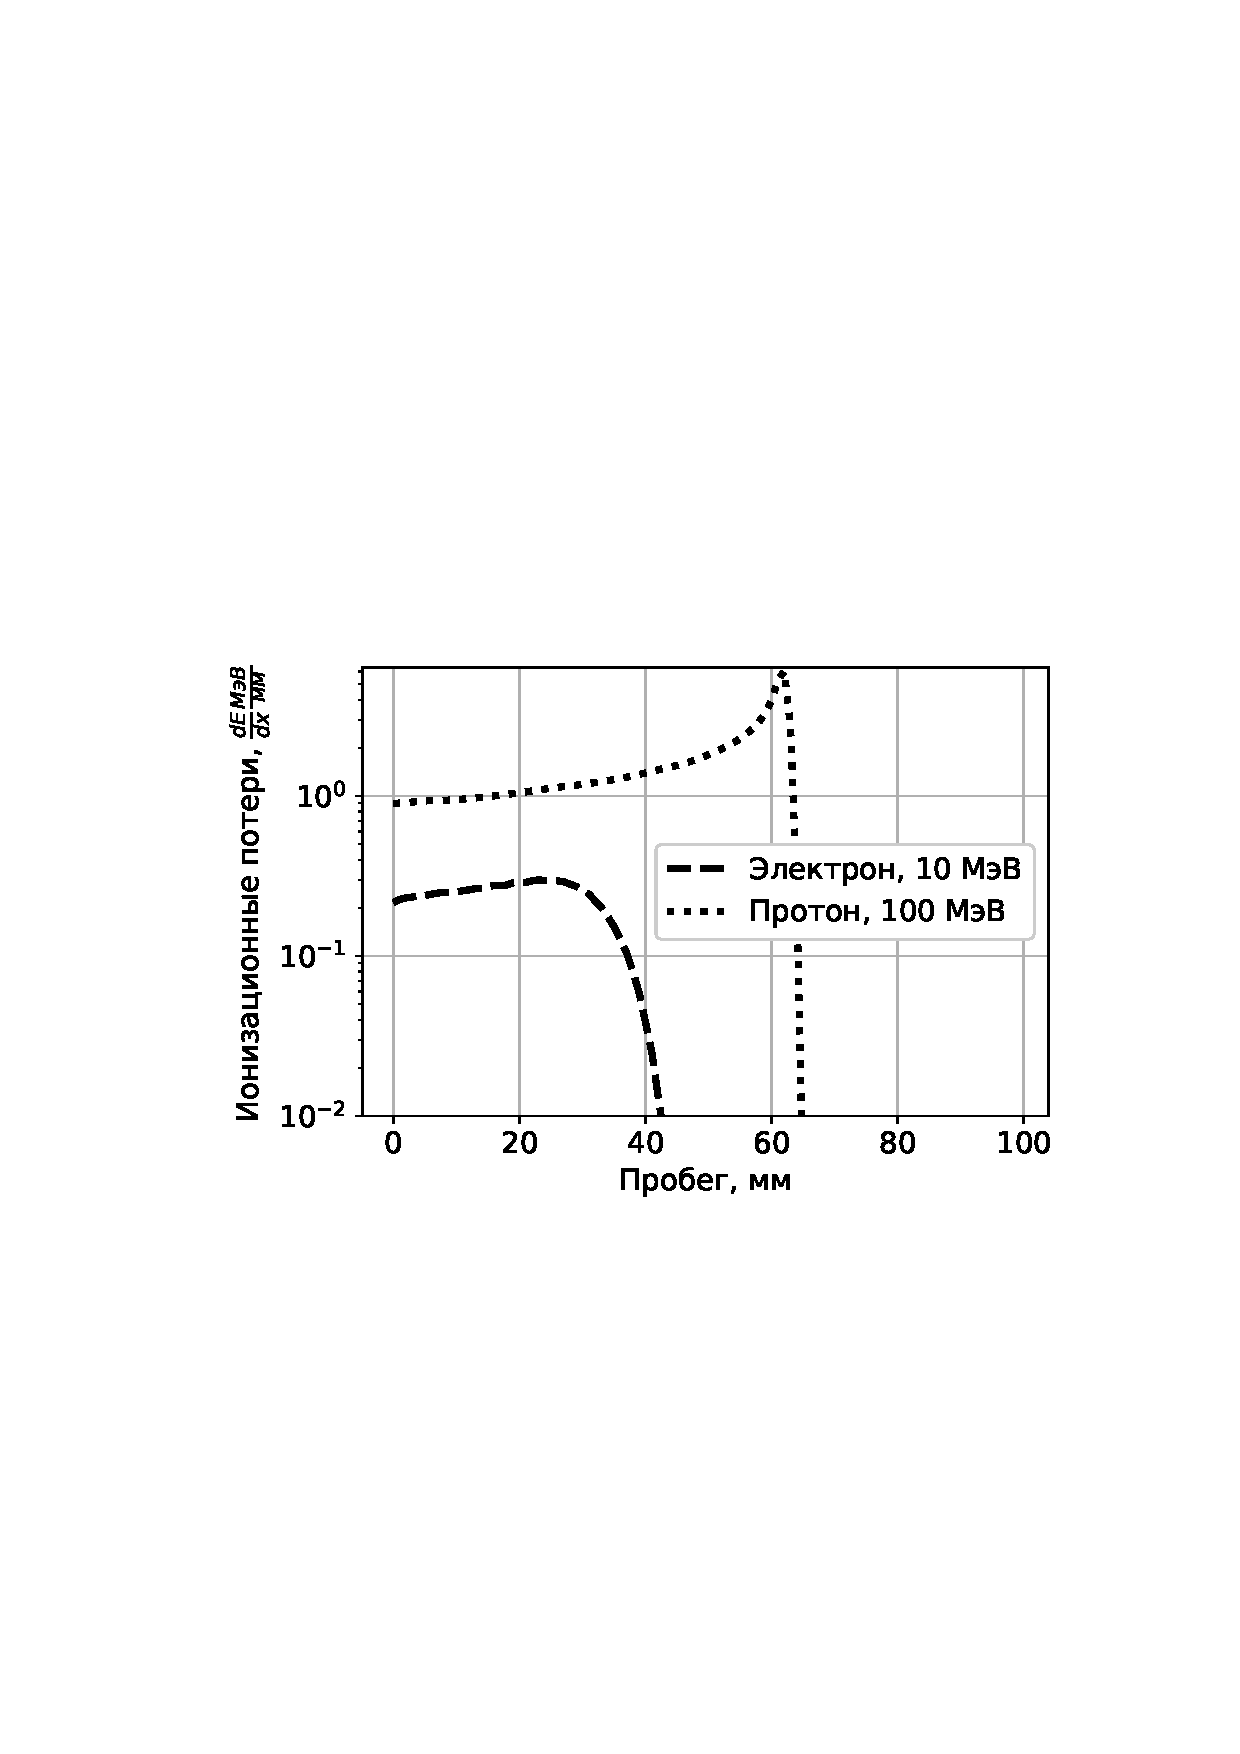
\includegraphics[width=0.95\linewidth]{pictures/01_bregg.pdf}
        \caption{}
        \label{pic-01-a}
    \end{subfigure}
	~
    \begin{subfigure}[b]{0.5\textwidth}
		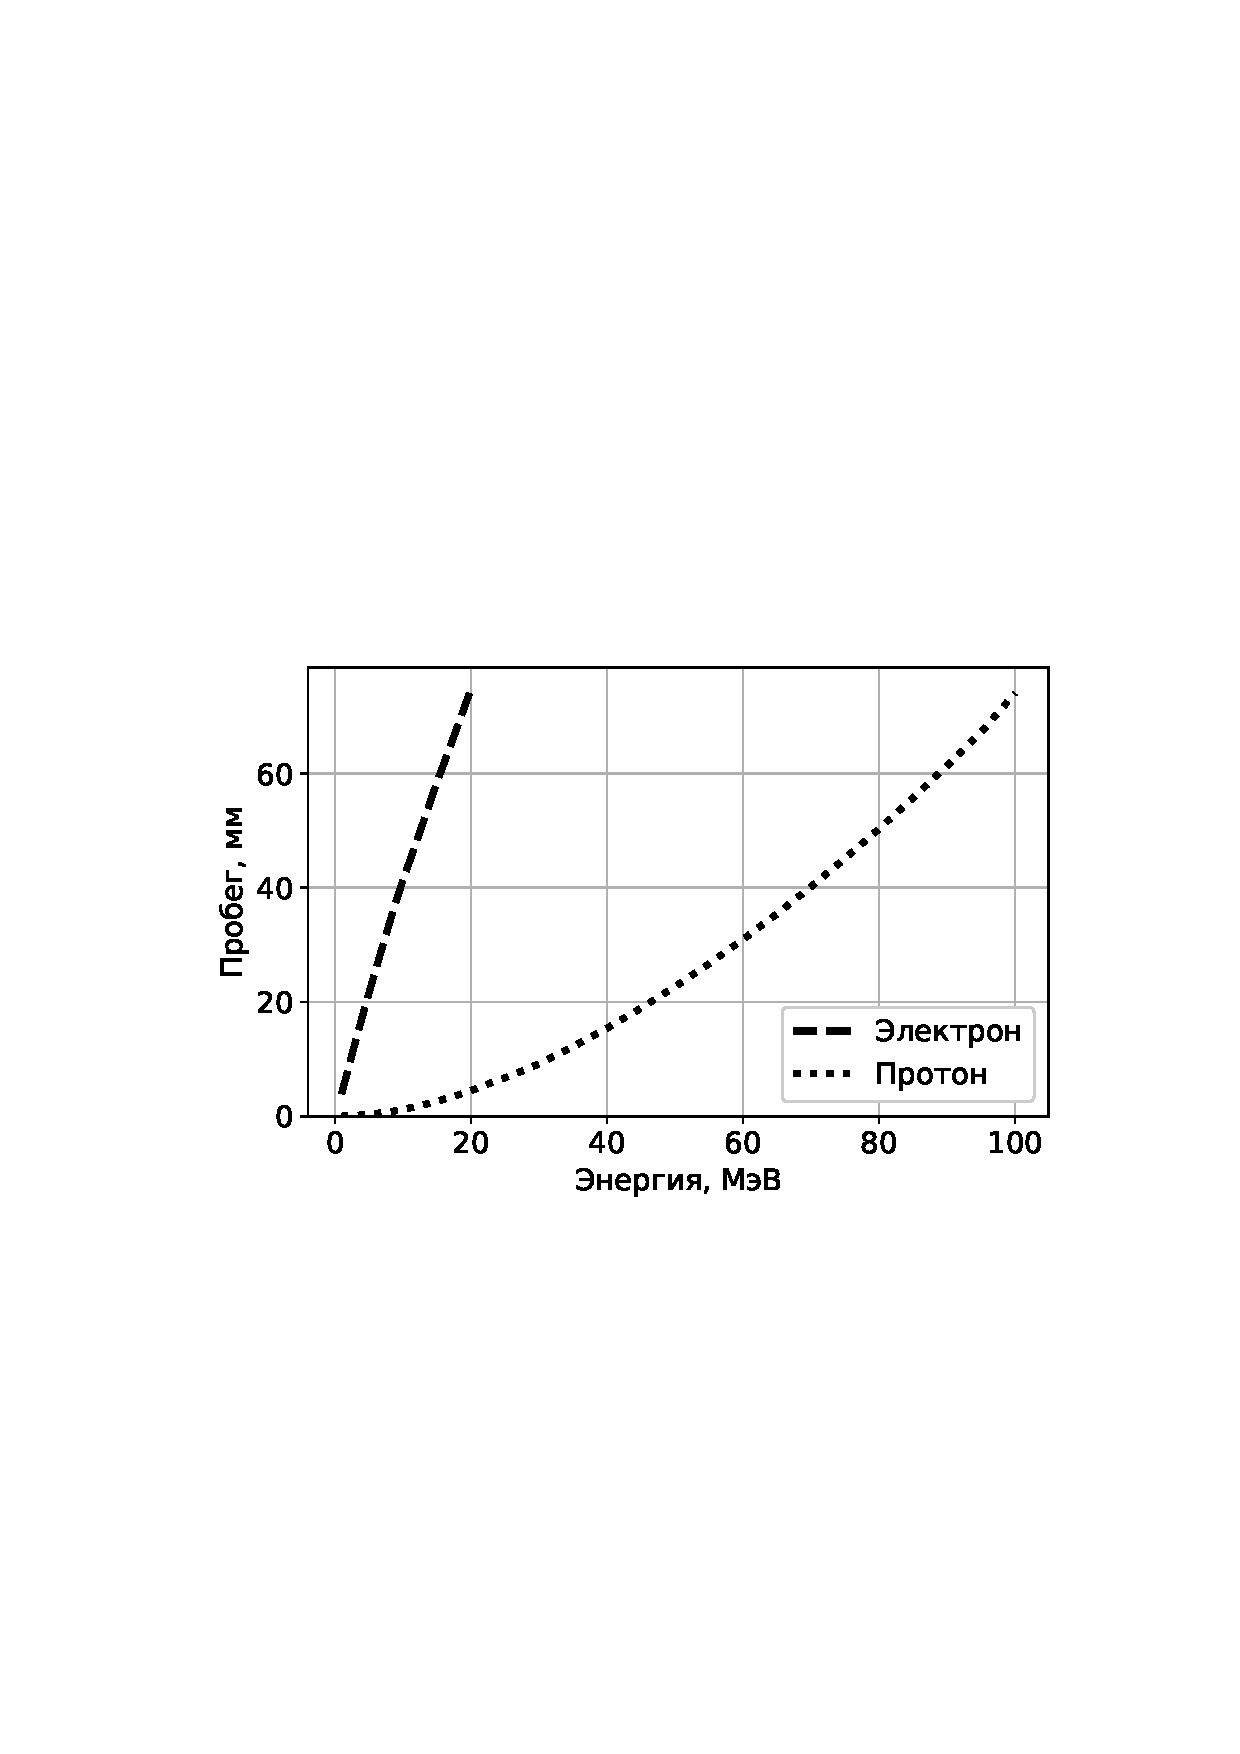
\includegraphics[width=0.95\textwidth]{pictures/02_range.pdf}
        \caption{}
        \label{pic-01-b}
    \end{subfigure}
    \caption{ a) Зависимость выделенной энергии от глубины для электрона и протона в антрацене. b) Полная длина пробега для протонов и электронов в антрацене}
\end{figure}

Телескоп представляет собой набор цилиндрических сцинтилляционных шайб, диаметром 2 -- 5~см, разделенных светоотражающим материалом  и помещенных в металлический корпус. В одном или нескольких местах в шайбе делается скос или “ушко” для установки фотоумножителя. Для обеспечения равномерного светосбора рассматриваются варианты с установкой до трех фотоумножителей на одну шайбу или с кольцевым оптоволокном. Места установки детекторов в последовательных шайбах могут быть сдвинуты относительно друг друга на $60^\circ$ для того, чтобы слои можно было делать достаточно тонкими и детекторы в соседних слоях не мешали друг другу. Входное окно телескопа остается открытым, но при необходимости на него может быть установлен коллиматор или фильтр низкоэнергетичных частиц (например, бериллиевое покрытие может отфильтровывать низкоэнергетичные протоны, при этом являясь прозрачным для электронов в  интересующем нас диапазоне энергий, из рис.~\ref{pic-02-a} следует, что оптимальным будет использовать напыление с толщиной 400 -- 500~мкм). Толщина шайб может быть выбрана разной в зависимости от конкретных задач детектора (более тонкие слои позволяют получить лучшее разрешение, но при этом увеличивается вес детекторов и сопутствующей электроники). В общем случае предполагается, что вблизи входного окна плотность слоев выше, поскольку там требуется большая точность определения формы кривой потерь (для идентификации электронов). Минимальная толщина может составлять от 2~мм. Вдали от входного окна толщина увеличивается и достигает 5 -- 10~мм. Полная толщина детектора может варьироваться в зависимости от необходимости снизить массу детектора или расширить диапазон регистрируемых энергий, так из рис.~\ref{pic-01-b} следует, что для полного поглощения протонов с энергией 100~МэВ требуется 65~мм антрацена. Корпус прибора частично обеспечивает пассивную защиту от боковых частиц (см. рис.~\ref{pic-02-b}), поглощая протоны с энергией 20~--~40~МэВ и электроны до 4~МэВ.
\begin{figure}[ht!]
	\begin{subfigure}[b]{0.5\textwidth}
    	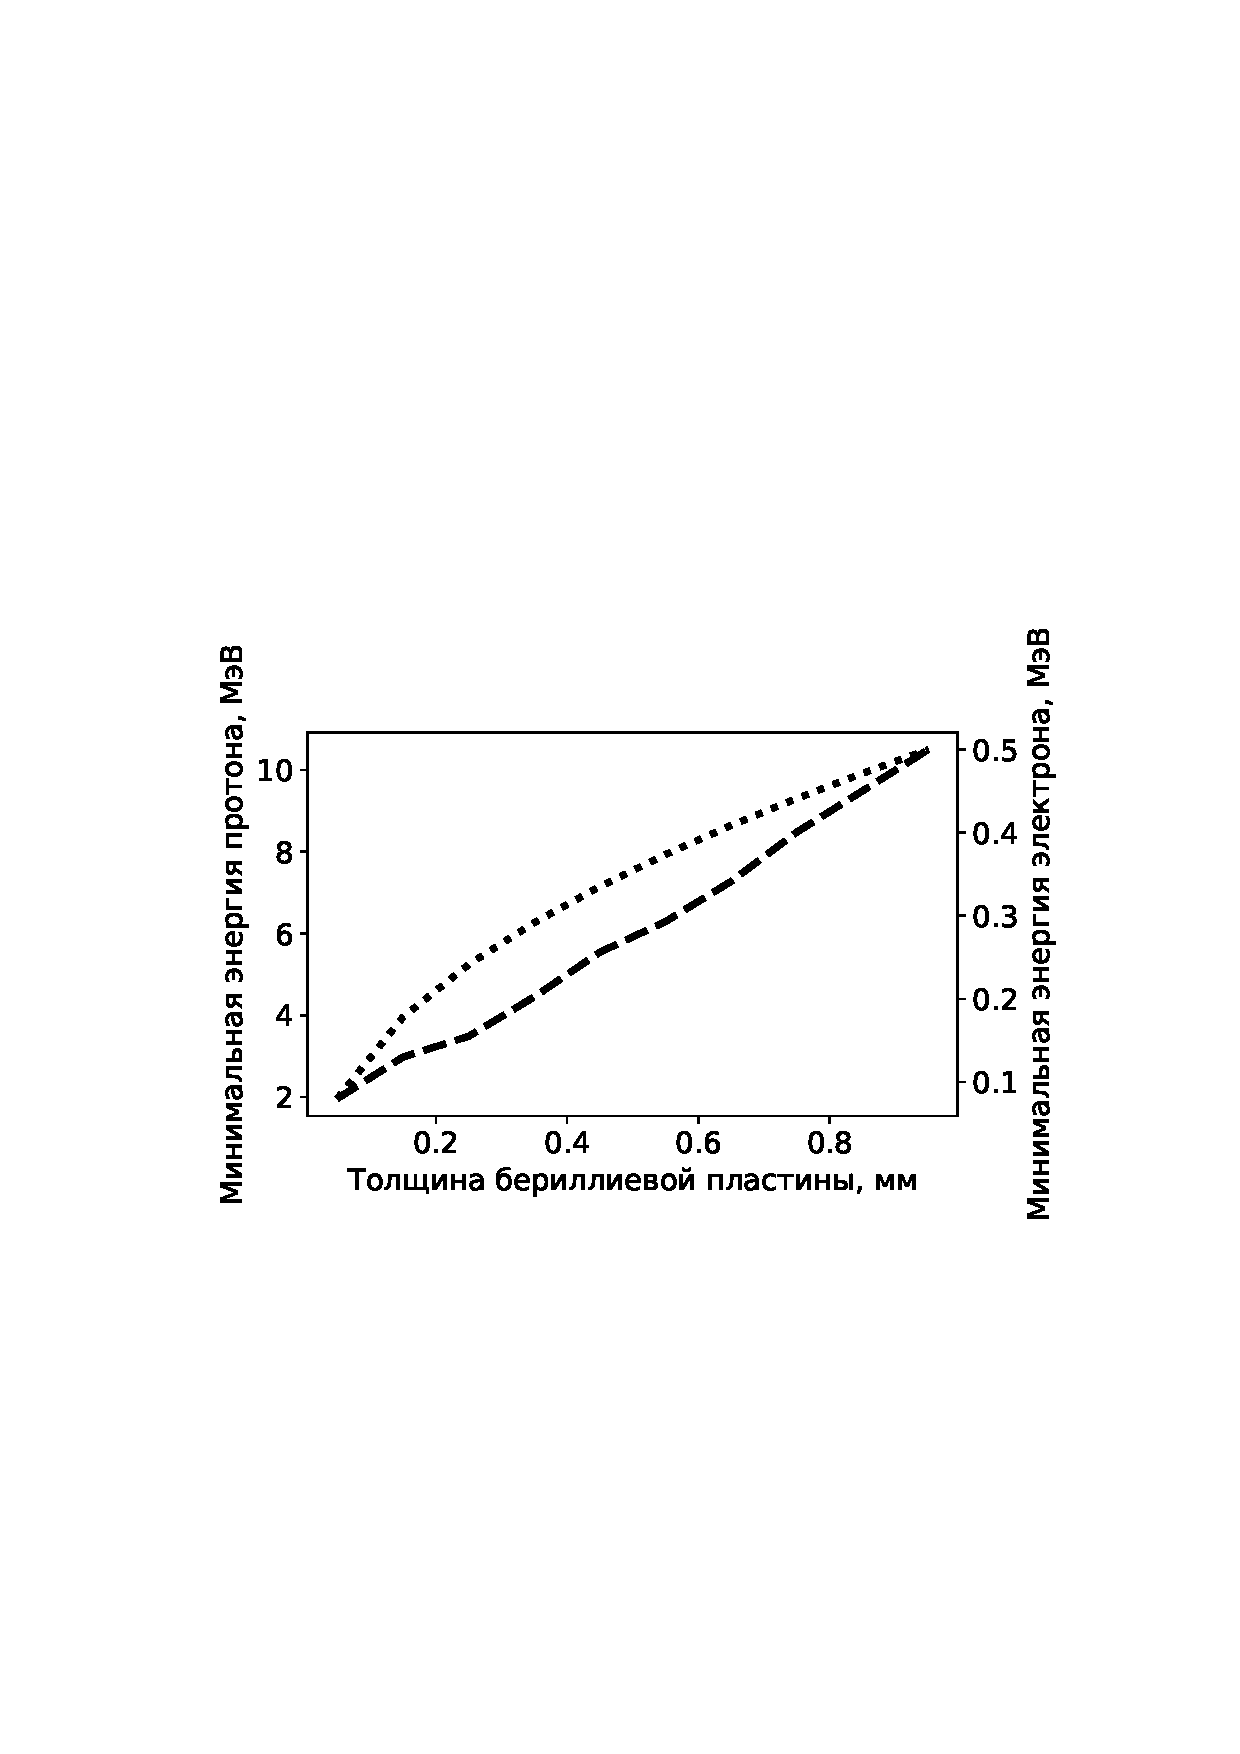
\includegraphics[width=0.95\linewidth]{pictures/03_berillium.pdf}
        \caption{}
        \label{pic-02-a}
    \end{subfigure}
	~
    \begin{subfigure}[b]{0.5\textwidth}
		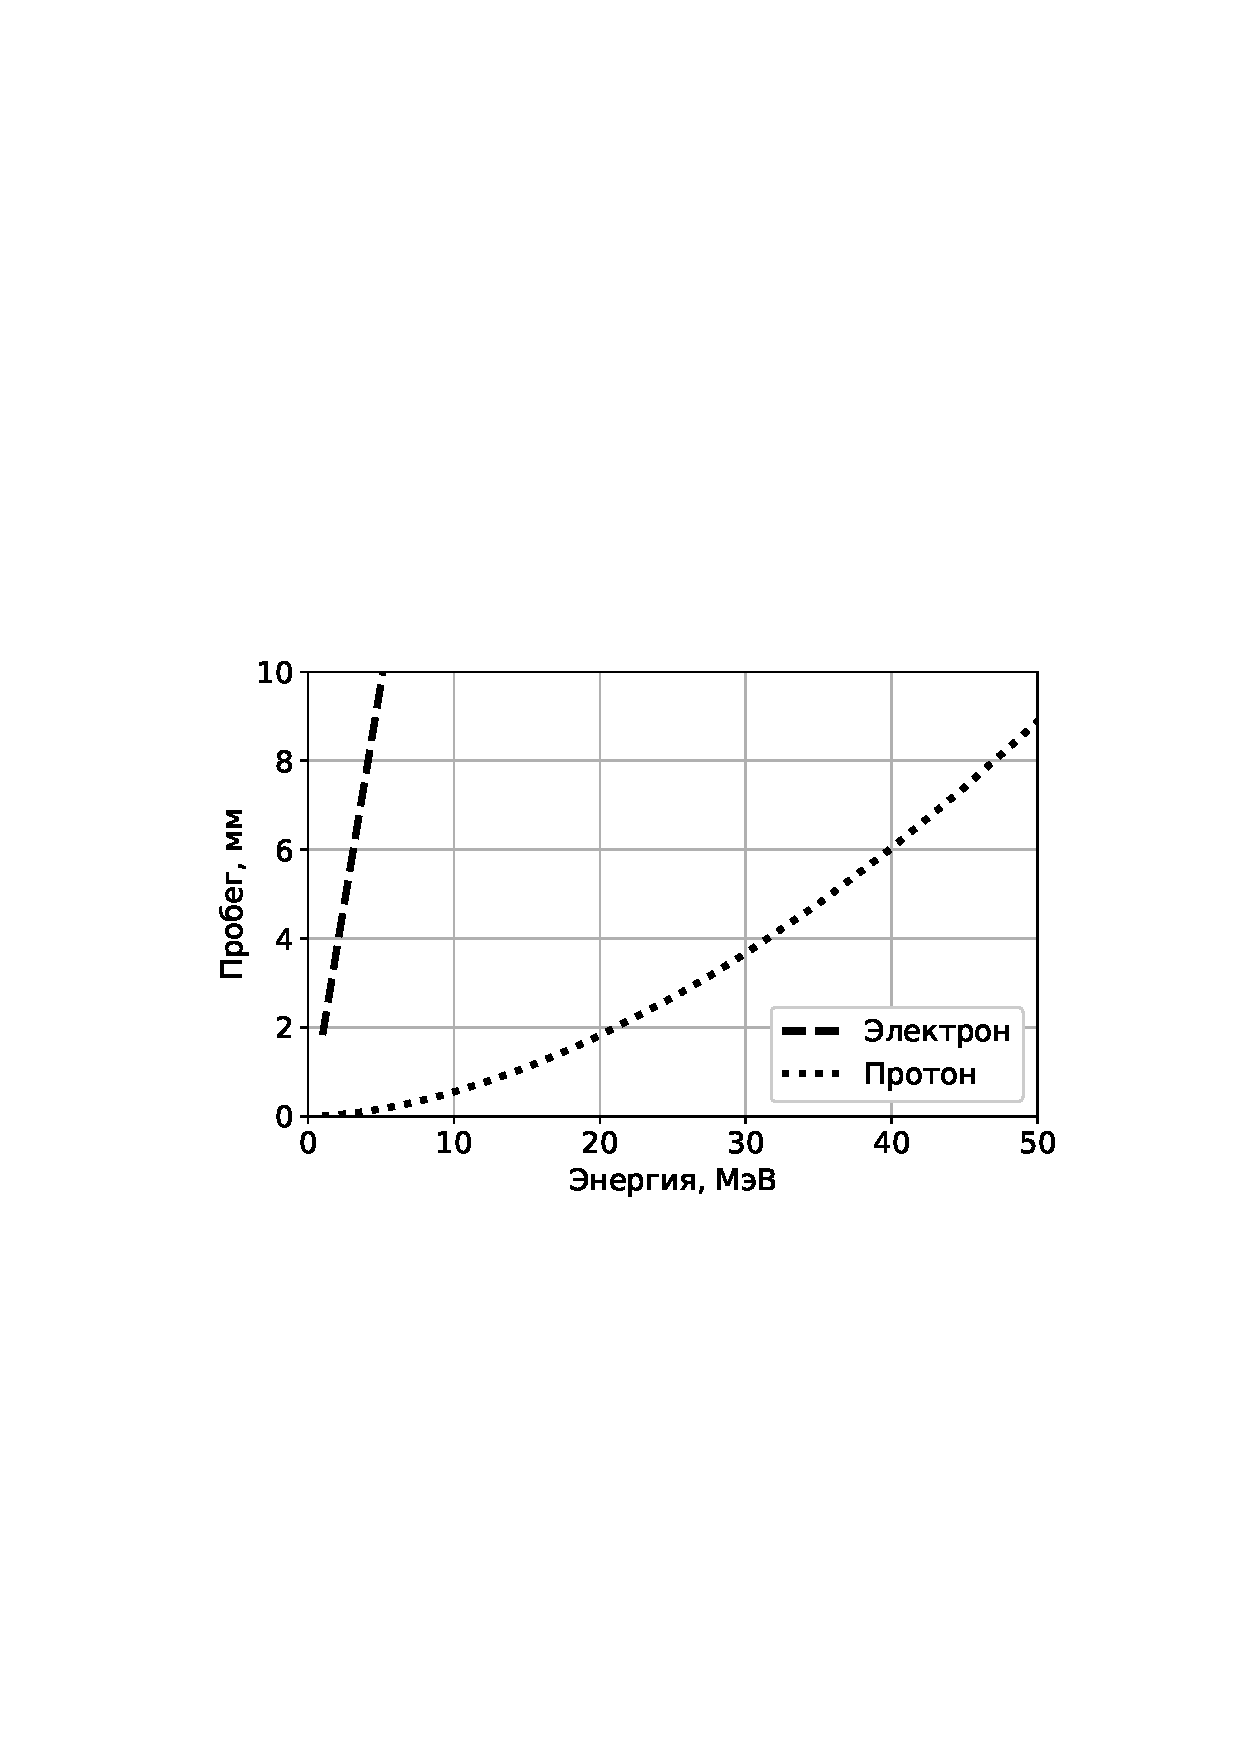
\includegraphics[width=0.95\textwidth]{pictures/04_casing.pdf}
        \caption{}
        \label{pic-02-b}
    \end{subfigure}
    \caption{ a) Минимальная энергия частицы для преодоления бериллиевого фильтра b) Полная длина пробега для протонов и электронов в D16}
\end{figure}

\section*{Моделирование и методика анализа.}
Из-за нестабильности величины потока солнечных частиц для детектора предусмотрены три режима работы. В первом режиме (при низкой скорости счета) производится анализ каждого события. Во втором режиме (при превышении некоторого порога, обусловленного скоростью работы электроники и временем высвечивания сцинтиллятора) идет накопление суммарного сигнала за некоторый промежуток времени, а затем восстанавливается энергетический спектр частиц, попавших в детектор за это время. Третий режим является смешанным: в шайбах, расположенных вблизи входного окна, проводится измерение суммарных ионизационных потерь, а в дальних шайбах --- идентификация отдельных событий. В качестве основы для анализа используются рассчитанные значения ионизационных потерь и набор триггеров для отсечения событий. Для расчета энерговыделения в сцинтилляционных шайбах проведено Монте-Карло моделирование при помощи транспортного кода GEANT4 ~\cite{ALLISON2016186}.  В качестве физической модели использовался модуль стандартной электромагнитной физики GeEmStandartPhysics, включающий в себя описание процессов, оказывающих основное влияние на распространение частиц в детекторе: ионизационные потери и их флуктуации, упругое кулоновское рассеяние и тормозное излучение электронов.

В одночастичном режиме для анализа отбираются события, прошедшие через входное окно, и, исходя из полной измеренной энергии и количества сработавших слоев, определяются диапазоны возможных параметров частицы, а также отсекаются события, пришедшие под большими углами. В данных диапазонах определяется набор параметров, максимизирующий значение функции правдоподобия --- произведения вероятностей наблюдать измеренное энерговыделение при данном наборе параметров. Предварительный алгоритм позволяет определить энергию протонов с точностью 1~МэВ для исходной энергии 50~МэВ, то есть дает точность порядка 2\%.

Для анализа спектра в интегральном режиме разрабатывается процедура, основанная на методике регуляризации обратных задач, разработанной В. Ф. Турчиным ~\cite{Turchin-epf}. 



Предварительный (неоптимизированный) результат применения процедуры для восстановления данных, имитирующих лобовой пучок протонов в детекторе из 20 сегментов (10 сегментов по 2~мм, 5 по 3~мм и 5 по 5~мм), приведен на рис.~\ref{pic-03-b}, пример референтной кривой поглощения в одном сегменте детектора,используемой для восстановления спектра, приведен на рис.~\ref{pic-03-a}. 

\begin{figure}[ht!]
	\begin{subfigure}[b]{0.5\textwidth}
    	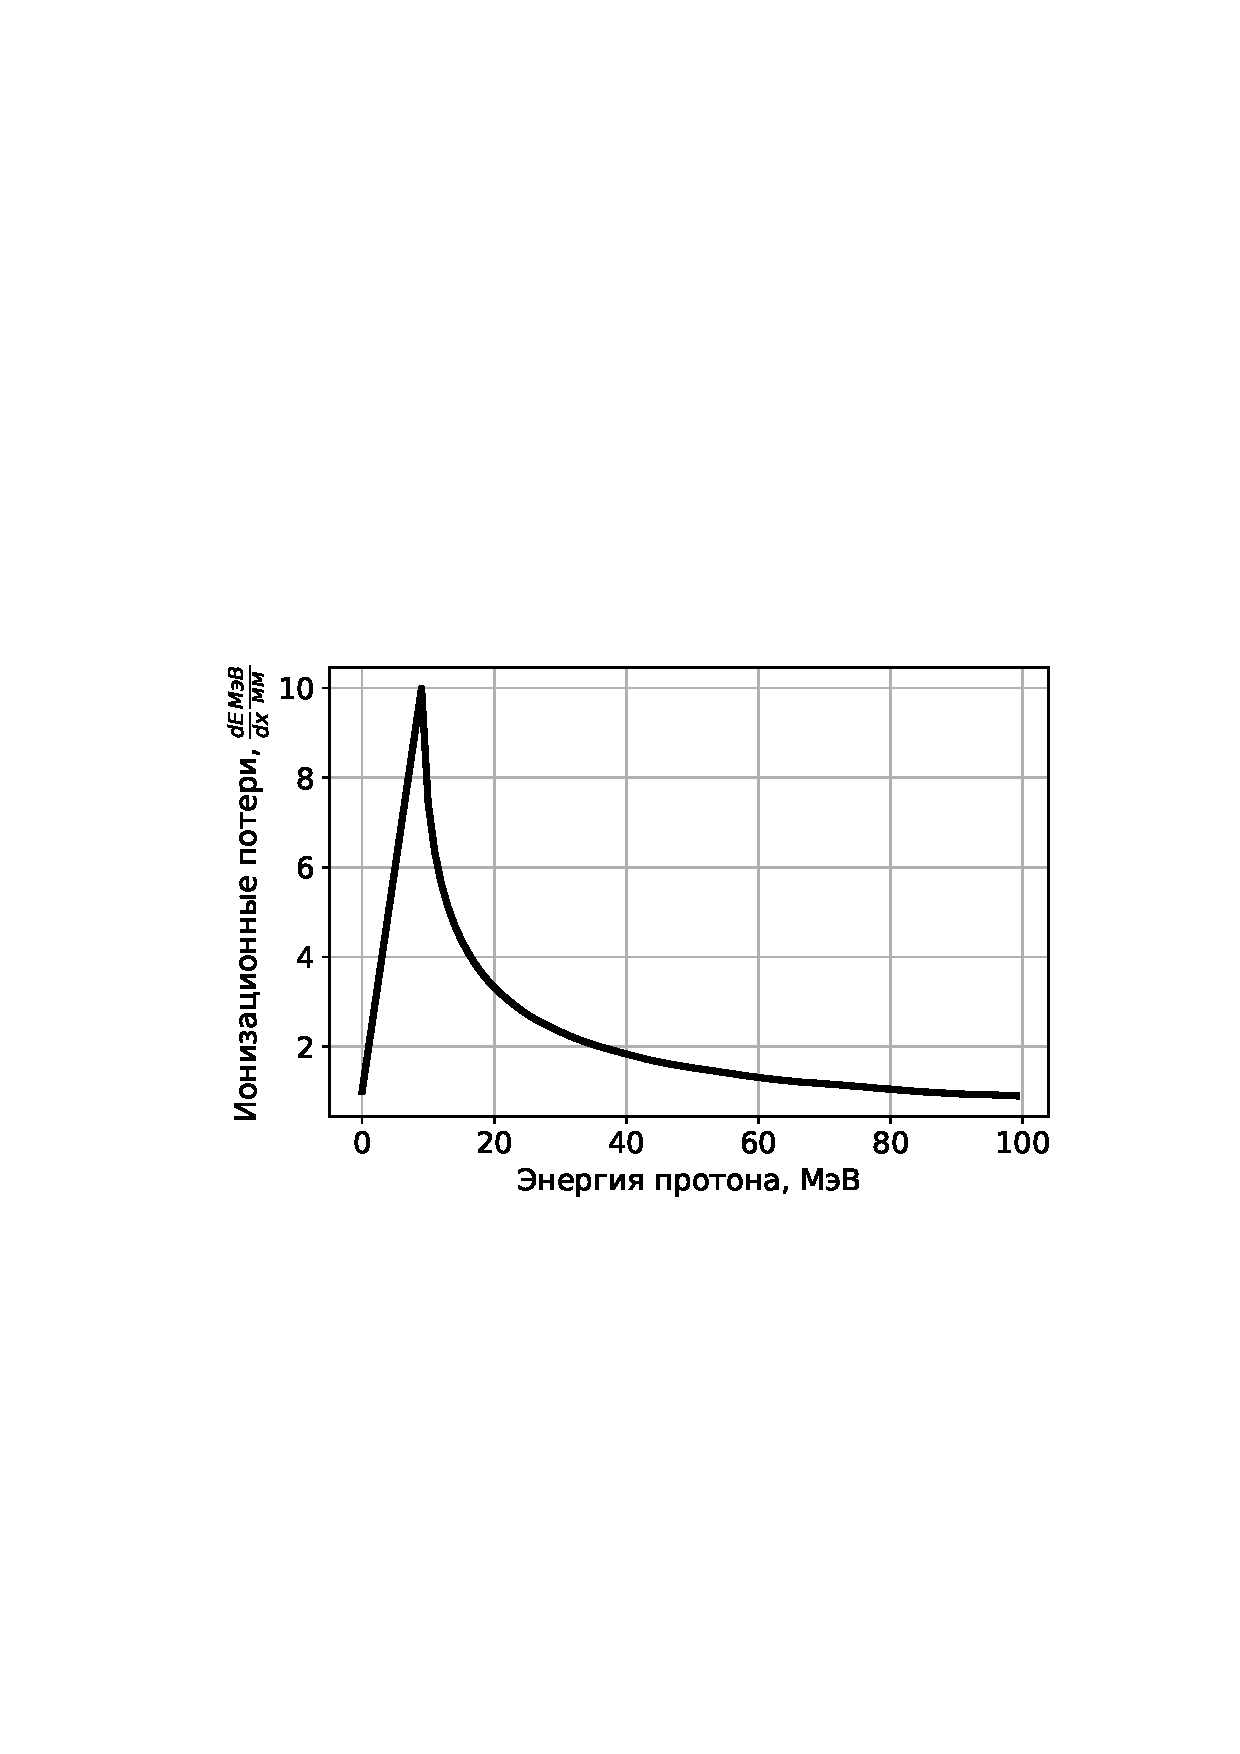
\includegraphics[width=0.95\linewidth]{pictures/05_LossInCell.pdf}
        \caption{}
        \label{pic-03-a}
    \end{subfigure}
	~
    \begin{subfigure}[b]{0.5\textwidth}
		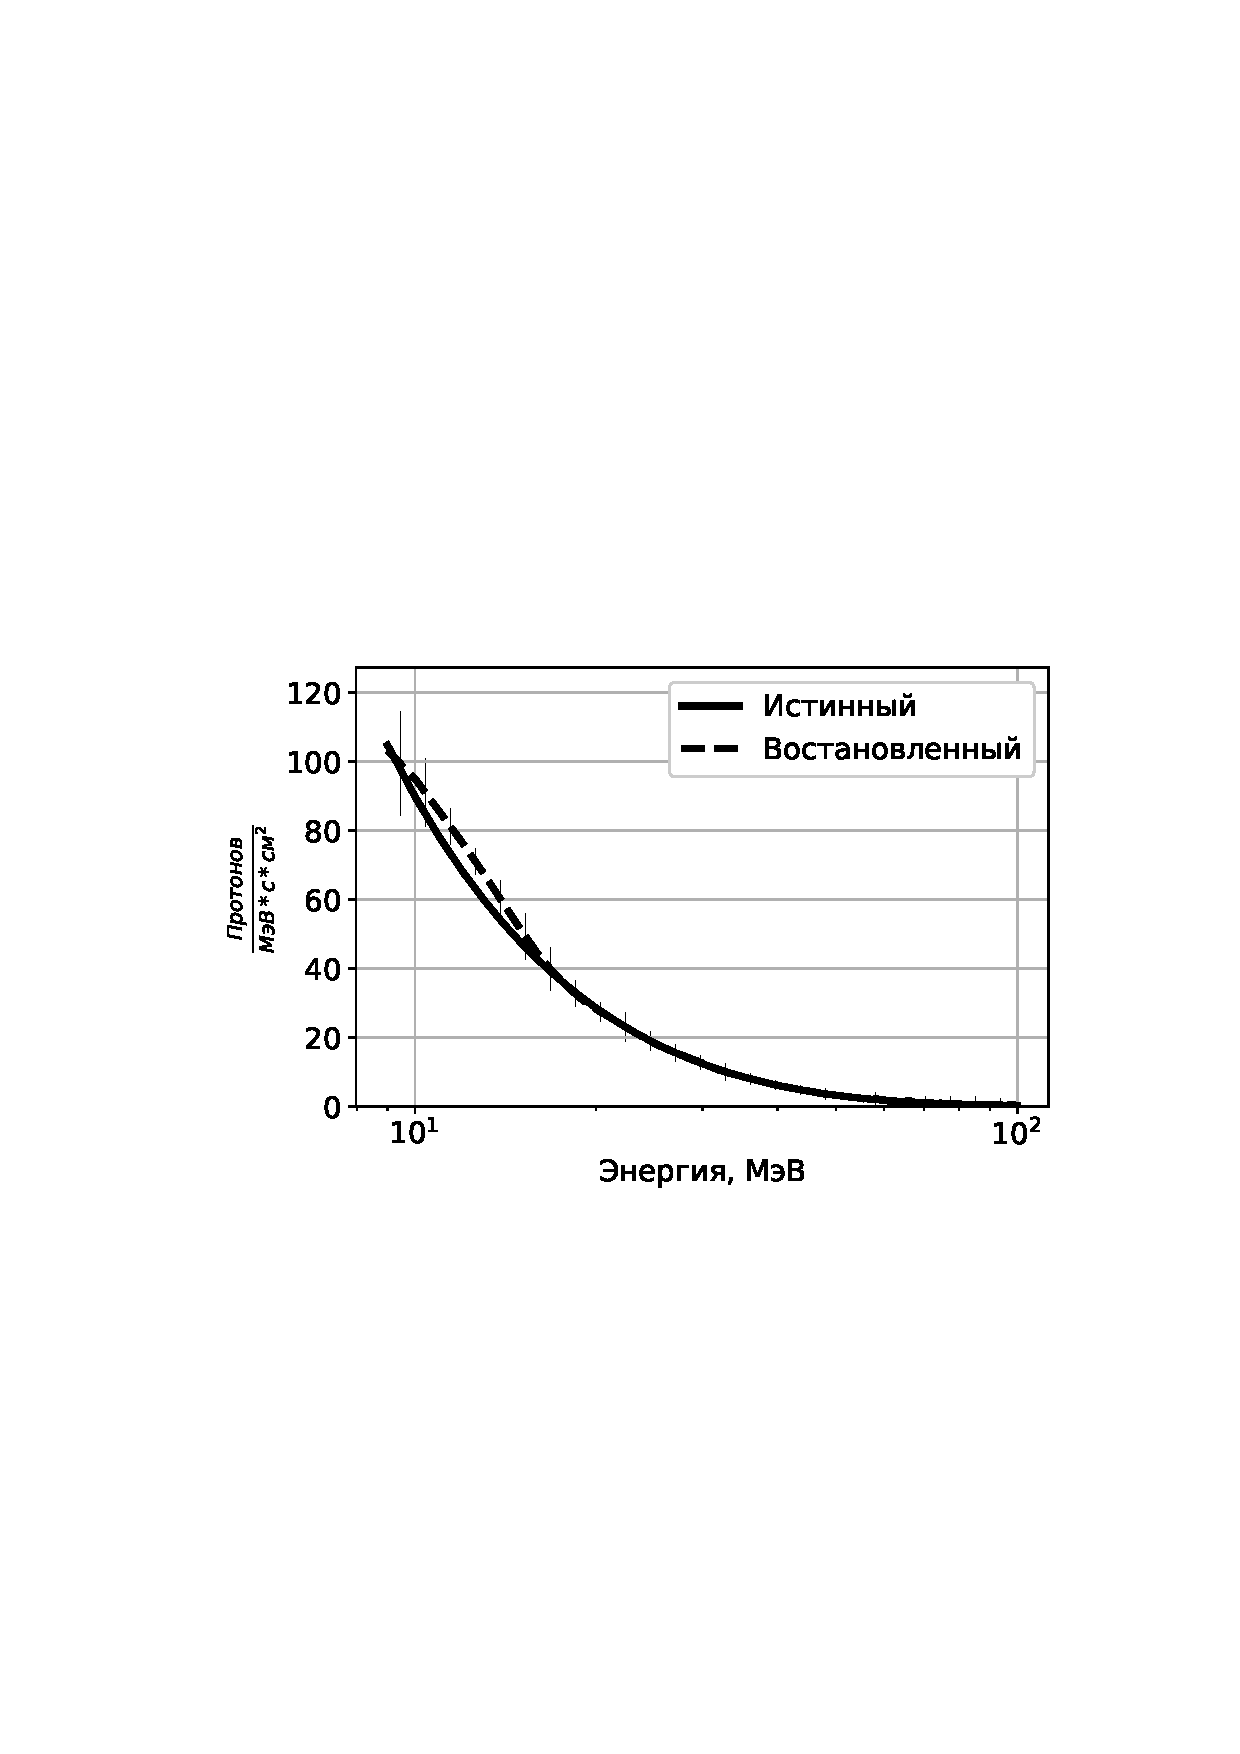
\includegraphics[width=0.95\textwidth]{pictures/06_IntegralSpectrum.pdf}

        \caption{}
        \label{pic-03-b}
    \end{subfigure}
    \caption{ a) Зависимость выделенной энергии от начальной энергии частицы в первом сегменте детектора. b) Результат восстановления дифференциального спектра.}
\end{figure}



\section*{Результаты.}
Разработана концепция секционного сцинтилляционного телескопа для регистрации высокоэнергетичных электронов и протонов солнечного происхождения. Произведены работы по моделированию детектора и сделаны оценки его чувствительности для различных частиц и в различных диапазонах энергий. Предварительные результаты показывают, что при весе до 1~кг детектор сможет позволить измерение энергетического спектра протонов от 5 до 100~МэВ и электронов от 1 до 10~МэВ с точностью порядка 1 -- 5\%.

Существенным преимуществом детектора является возможность работы в так называемом интегральном режиме, когда не регистрируются индивидуальные частицы, а идет анализ полного пространственного спектра потерь энергии. Интегральный режим позволяет работать при скоростях счета более 1~МГц, обеспечивая при этом достаточно хорошую (около 5\%) точность восстановления исходного спектра и состава излучения.

\section*{Благодарности.}
Исследование выполнено за счет гранта Российского научного фонда (проект № 17-72-20134).


\begin{thebibliography}{5}
    \bibitem{Turchin-epf}  M. Zelenyi, M. Poliakova, A. Nozik, A. Khudyakov,  in Proceedings of the XXI International Scientific Conference of Young Scientists and Specialists, Dиbna, Russia, 2017,  \href{https://doi.org/10.1051/epjconf/201817707005}.
    \bibitem{Gruppen} C. Grupen, B. Shwartz, Particle Detectors (Cambridge University Press, 2008).
    \bibitem{ALLISON2016186} J. Allison at el., Nuclear Instruments and Methods in Physics Research Section A: Accelerators, Spectrometers, Detectors and Associated Equipment, 835, 186 - 225 (2016).  
    \bibitem{miroshnichenko2015solar} L. Miroshnichenko, Solar Cosmic Rays: Fundamentals and Applications, (Springer, 2015).
    \bibitem{petrukovich2008cosmic} А.А. Петрукович, А.В. Дмитриев, В.М. Петров, Плазменная гелиогеофизика, Т. II (Физматлит, 2008).
\end{thebibliography}

% Список терминов, сокращений и перевод
% Спорадические явления – sporadic phenomena
% Солнечная активность – solar activity
% Солнечная вспышка – solar flare
% Солнечные космические лучи (СКЛ) – solar cosmic rays (SCR)
% Галактические космические лучи (ГКЛ) – galactic cosmic rays (GCR)
% События наземных возрастаний (СНВ) – ground level events (GLE)
% Корональный выброс массы (КВМ) – coronal mass ejection (CME)
% Космический аппарат (КА) – spacecraft 
% Полупроводниковый детектор (ППД) – solid state detector (SSD)
% Фотоэлектронный умножитель (ФЭУ) – Photomultiplier (PMT) 
% Гелиосфера – Heliosphere
% Гелиодолгота - Heliolongitude
%%Конец введение от Ивана



\end{document}
